
As the charged Higgs boson decays to a charm and a strange antiquark, the
identification of charm jet is expected to increase the signal significance.
The charm tagging or \PQc tagging is recently developed in the CMS collaboration
\cite{CMS-PAS-BTV-16-001} based on the \verb|CSVv2| method for the analyses at 13 \TeV 
data. This procedure is similar to that of \PQb tagging described in 
Section~\ref{s:bTag}. At the end, we have two charm discriminators: \PQc vs. \PQb jet (\verb|CvsB|) 
and \PQc vs. light jet (\verb|CvsL|). These are collectively used 
to tag a jet as \PQc jet. There are three working points for the \PQc tagging as shown 
in Table~\ref{tab:cTagEff} and Figure~\ref{fig:cTagger}. Distribution of these two discriminators after
kinematic fit selection is shown in Figure~\ref{fig:pfCCvsBL} for the \mujets and \ejets channel. 
\begin{table}
\begin{center}
\caption{The efficiency of loose (L), medium (M), and tight (T) \PQc tag working points for
    different quark-flavor of jets \cite{Sirunyan:2017ezt}. These efficiencies 
    are calculated from \ttbar events with jet \pt $>$ 20 \GeV.}
\begin{tabular}{cccccc}
\hline
\hline
Working point & $\epsilon^c$ (\%) & $\epsilon^b$ (\%) & $\epsilon^{udsg}$ (\%) & \verb|pfCCvsL| & \verb|pfCBvsB|\\ \hline\hline
\PQc tagger L & 88 & 36 & 91 & $>$ -0.48 & $>$ -0.17 \\
\PQc tagger M & 40 & 17 & 19 & $>$ -0.1  & $>$  0.08 \\
\PQc tagger T & 19 & 20 & 1.2& $>$ 0.69  & $>$ -0.45 \\
\hline
\end{tabular}
\label{tab:cTagEff}
\end{center}
\end{table}
%ctag eff figure
\begin{figure}
\centering
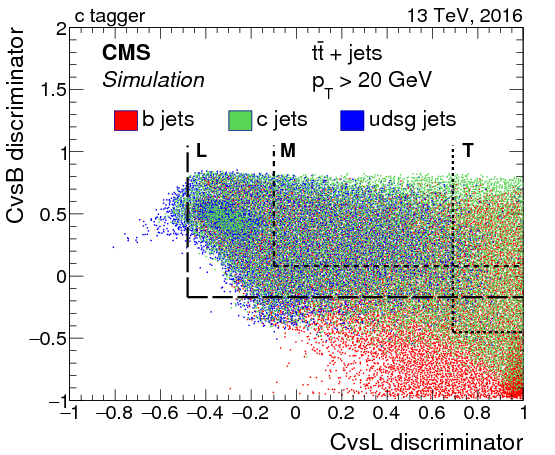
\includegraphics[width=0.5\linewidth]{Image/cTagger.png}
\caption{The 2D plot between the two \PQc taggers. The region right to the vertical 
    and above to the horizontal line correspond to different charm working 
    points (WPs). Unlike the \PQb tag WPs, there is an overlap between the loose,
    medium, and tight \PQc tag WPs. This figure is taken from ~\cite{CMS-PAS-BTV-16-001}.}
\label{fig:cTagger}
\end{figure}

\begin{center}
\begin{figure}
\subfigure[\PQc vs. \PQb jet discriminator ]{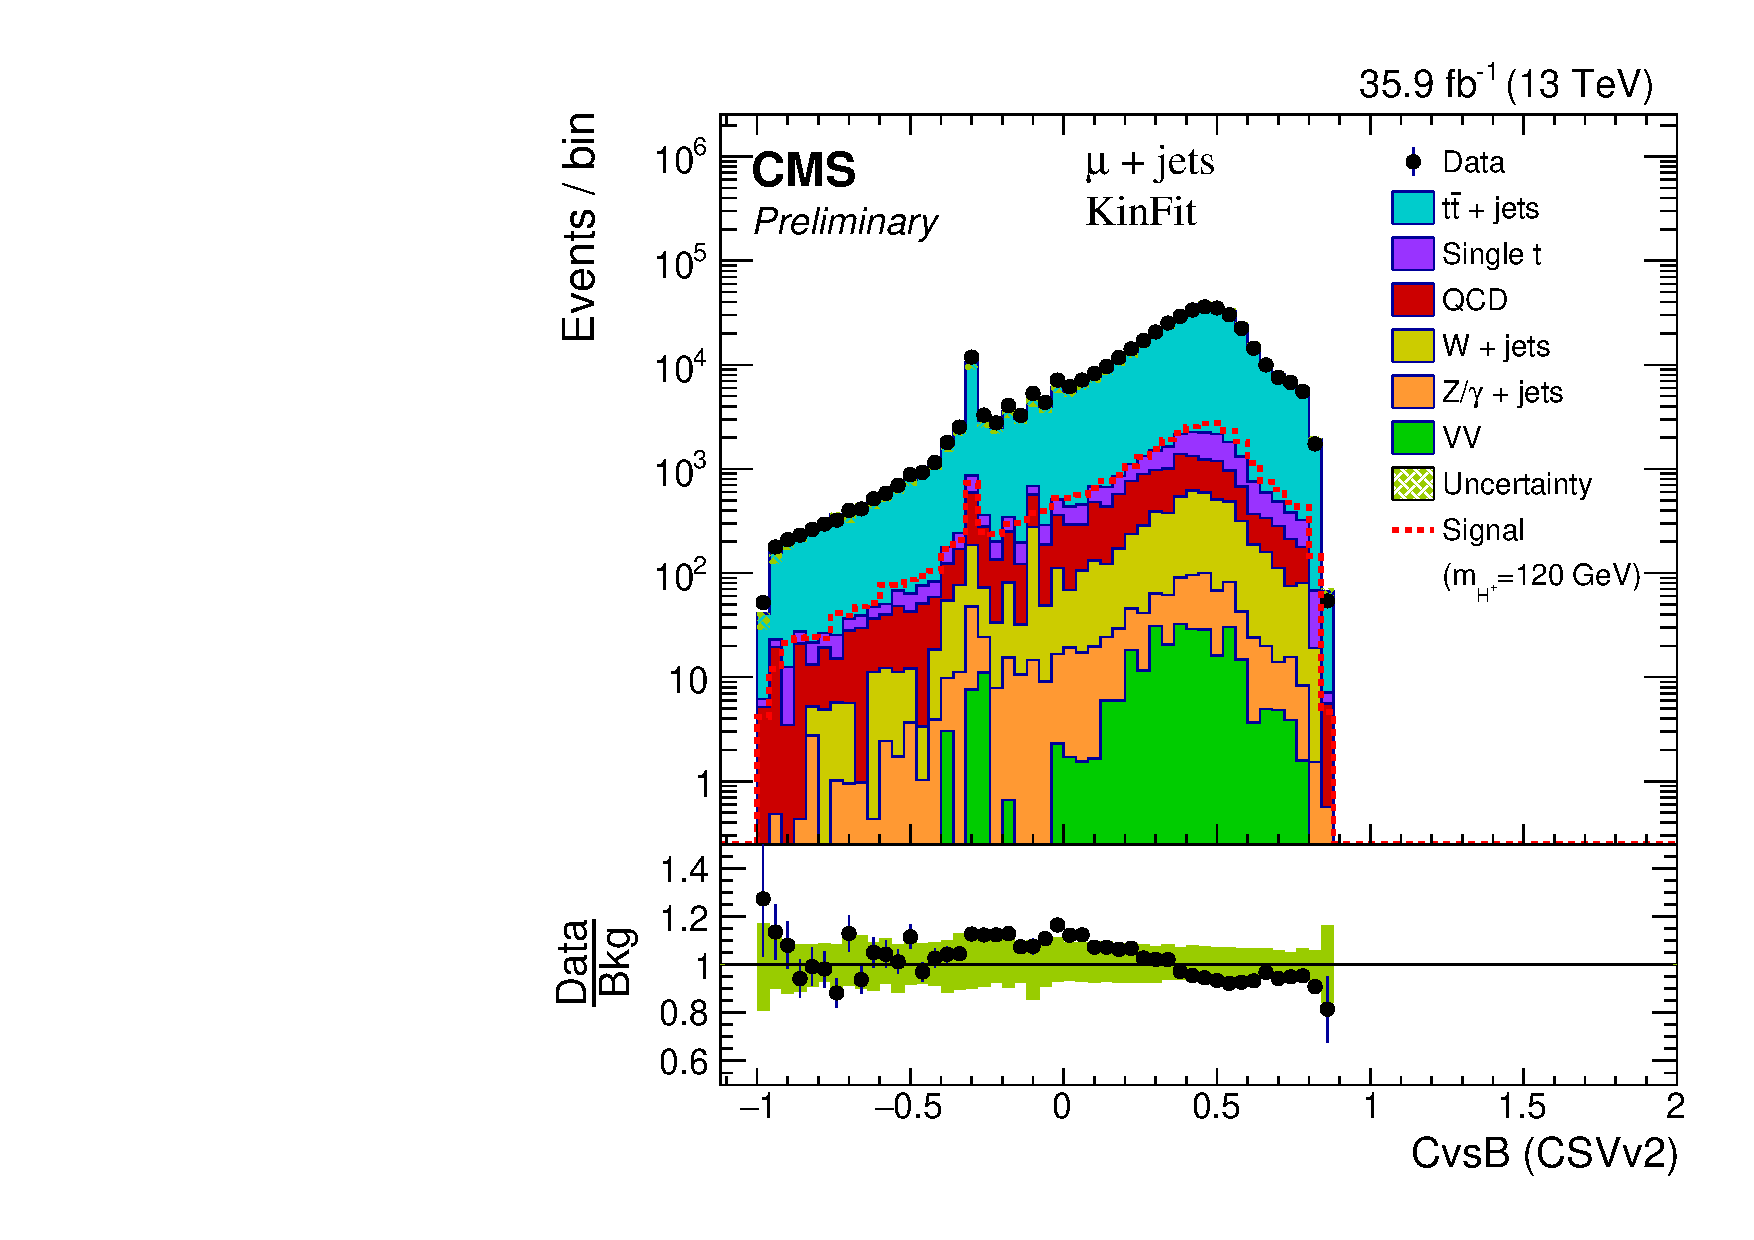
\includegraphics[width=0.50\linewidth]{Image/Muon/KinFit/pfCCvsB_muKinFit.pdf}}
\subfigure[\PQc vs. \PQb jet discriminator ]{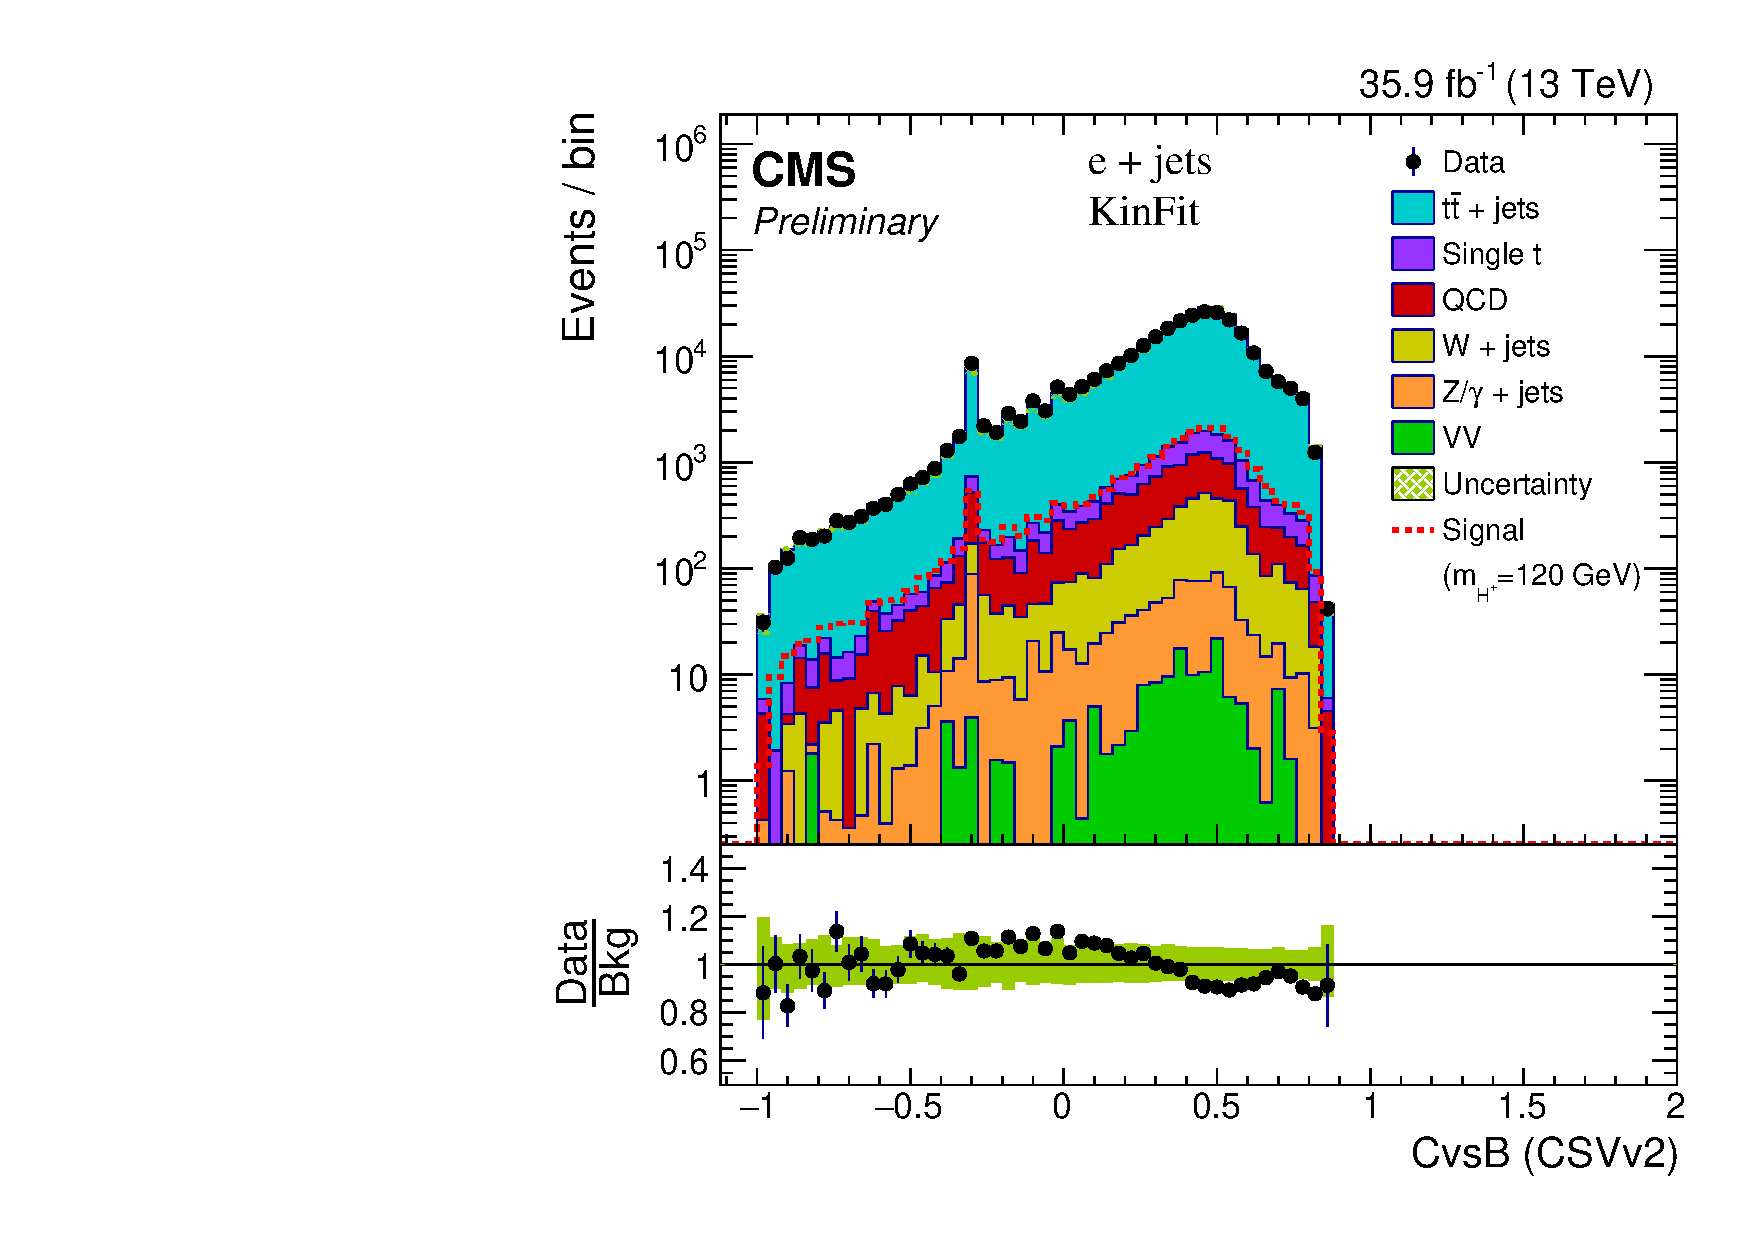
\includegraphics[width=0.50\linewidth]{Image/Electron/KinFit/pfCCvsB_eleKinFit.pdf}}
\vfil
\subfigure[\PQc vs. light jet discriminator ]{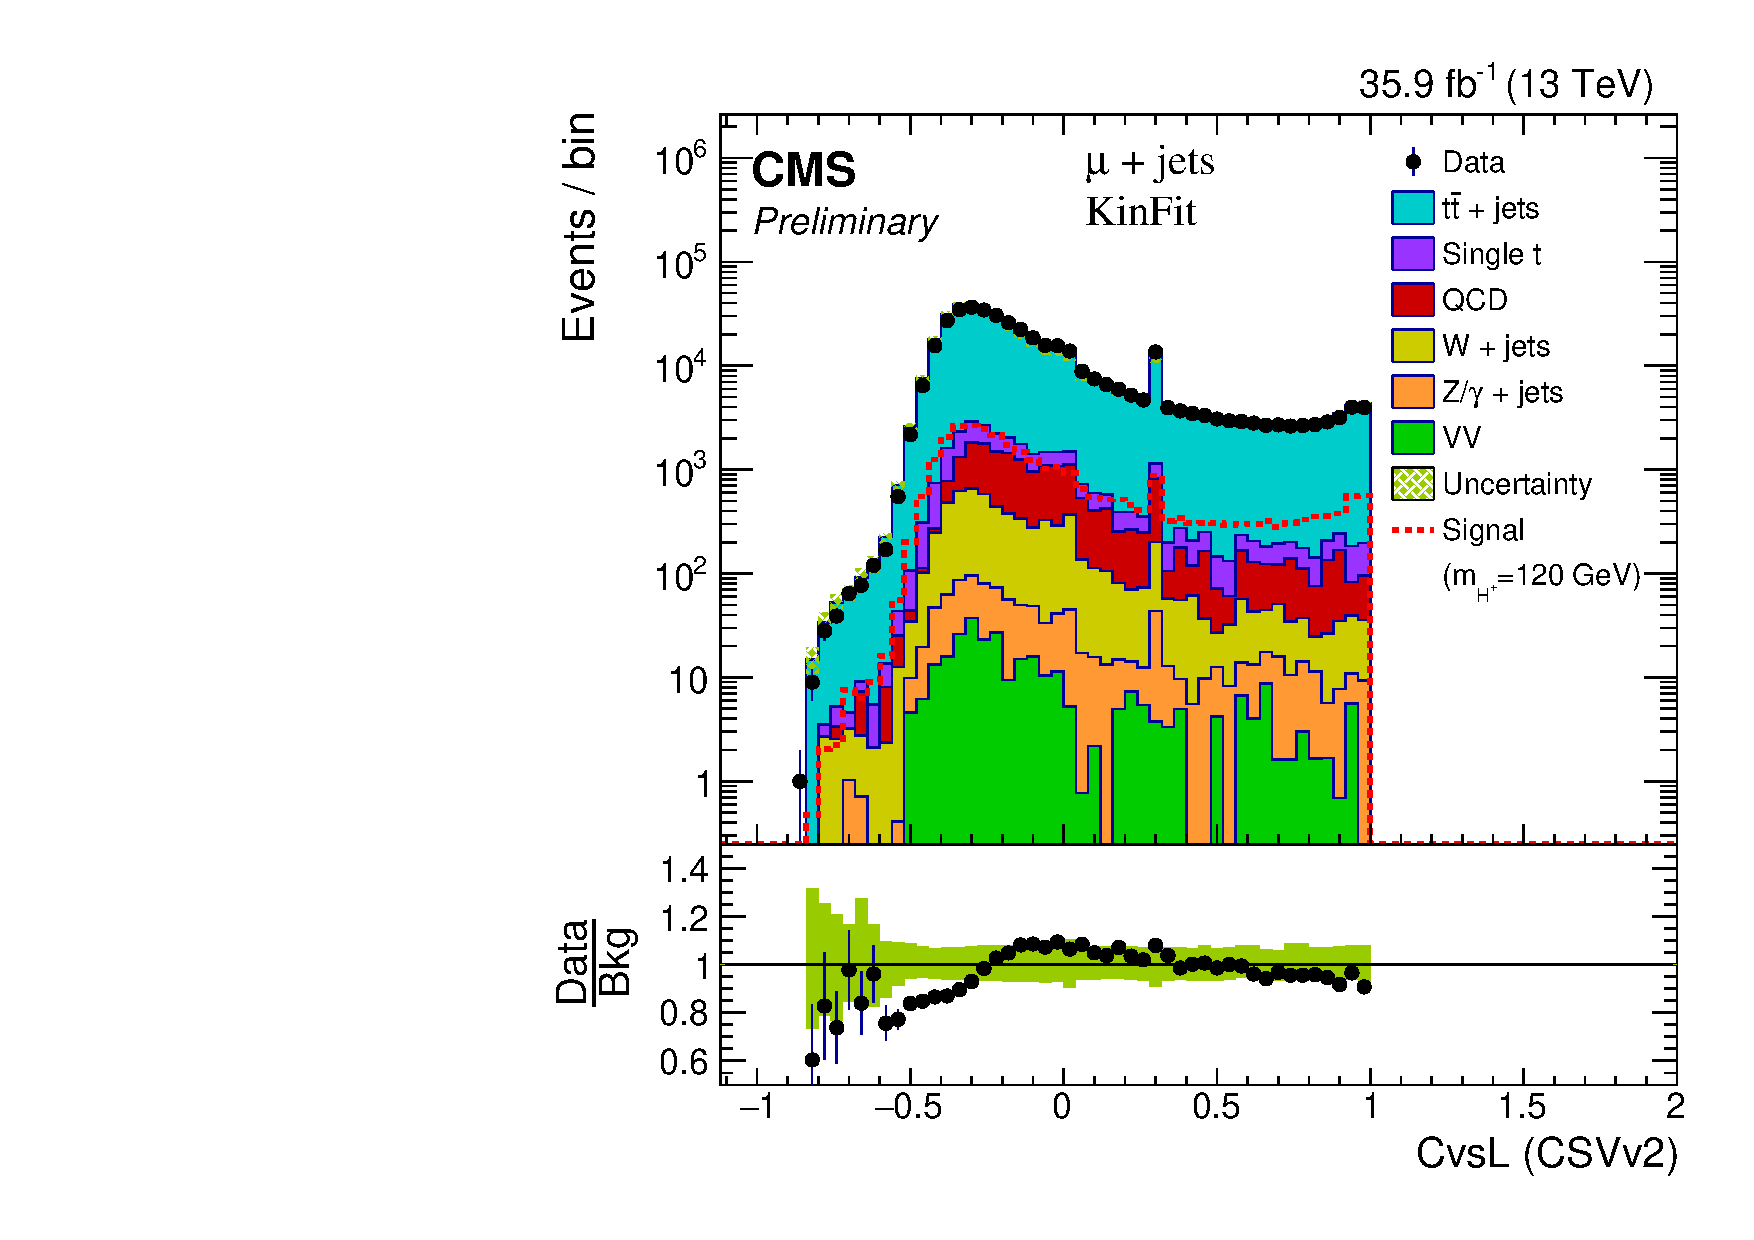
\includegraphics[width=0.50\linewidth]{Image/Muon/KinFit/pfCCvsL_muKinFit.pdf}}
\subfigure[\PQc vs. light jet discriminator ]{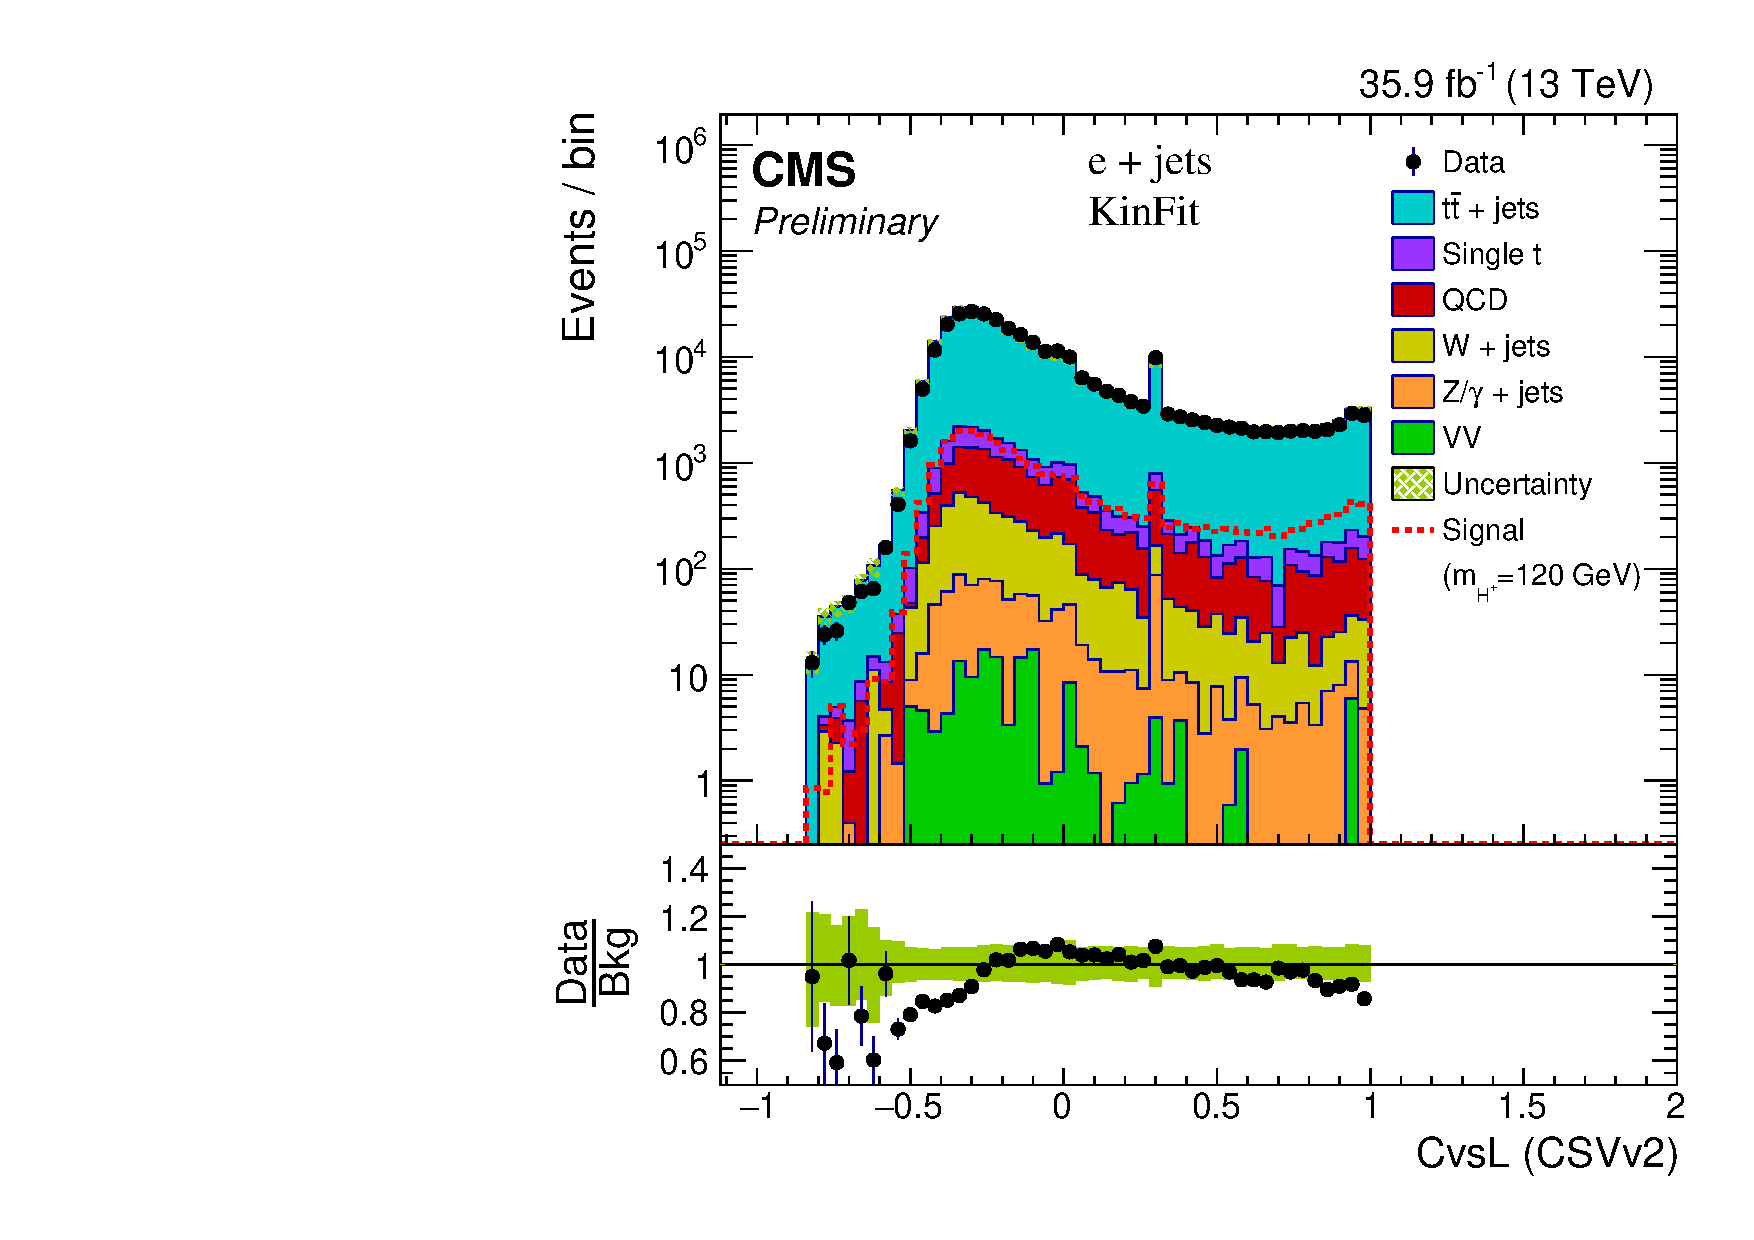
\includegraphics[width=0.50\linewidth]{Image/Electron/KinFit/pfCCvsL_eleKinFit.pdf}}
\caption{ The \PQc discriminator distribution of two non \PQb jets after 
    kinematic fitting selection for \mujets and \ejets channel.} 
\label{fig:pfCCvsBL}
\end{figure}
\end{center}


\section{\text{c} tag scale factor and selection}
\label{s:cTagSF}
Similar to the event weights for \PQb tagging, the event weight for \PQc jet tagging is also 
applied due to the mismatch in the efficiencies between simulation and data. The mistagging of 
\PQc-tagged jet or tagging a non \PQc tagged jet as \PQc jet is done using the same
procedure as that of Section~\ref{s:bTagSF}. The \PQc tagging requirement is applied on the two 
light jets from the kinematic fit. Event yield after demanding at least one \PQc-tagged jet with 
the loose working point for signal, background, and data are shown in 8th column of 
Tables~\ref{tab:cutflow_mu}, \ref{tab:cutflow_ele}, \ref{tab:cutflow_mu_sig} and 
\ref{tab:cutflow_ele_sig}. The \mjj distribution for the loose \PQc tagging is shown in
Figure~\ref{fig:mjj_cTagL}.

Initially, each working point was separately used for \PQc tagging. However, the 
limits were not getting improved for medium and tight working points. Therefore the 
loose working is finally used. Although the signal to background ratio increases as 
one go from loose to tight working points, 
the limits are not improved because the event yield also goes down. However,
it is found that, as described in Section~\ref{ss:mjj_cTagEx}, that if the 
events after kinematic fit selection are \textit{exclusively} divided into the categories 
based on loose, medium, and the tight charm working points and the limit is 
computed by combining the \mjj distributions from these three categories, as described in 
Section~\ref{ss:limit_cTagEx}, then the limit gets improved.


